\documentclass{article}
\usepackage[margin=1in]{geometry}
\usepackage{enumitem}
\usepackage{setspace}
\usepackage{amsmath}
\usepackage{amssymb}
\usepackage{physics}
\usepackage{graphicx}

\title{Math 180 Homework 3}
\date{10/22/2020}
\author{Jiaping Zeng}

\begin{document}
\setstretch{1.35}
\maketitle

\begin{itemize}
      \item [6.2.1] Show that the graph $K_{3,3}$ is not planar, in a manner similar to the proof of nonpolarity of $K_5$ given in the text.\\
            \textbf{Answer}: By contradiction; let $b_1,b_2,b_3$ and $b_4,b_5,b_6$ be the vertices of the two opposing sets of vertices, in addition let the arc connecting the points $b_i$ and $b_j$ be denoted by $\alpha(i,j)$.\\
            Since $b_1,b_2,b_4,b_5$ forms a cycle, the arcs $\alpha(1,4),\alpha(4,2),\alpha(2,5)$ and $\alpha(5,1)$ form a Jordan curve $k$, and hence the points $b_3$ and $b_6$ lie either both inside or both outside $k$, otherwise the arc $\alpha(3,6)$ would cross $k$.\\
            Suppose that $b_3$ lies inside $k$ (which divides $k$ into two Jordan curves) and $b_6$ lies inside the Jordan curve formed by the arcs $\alpha(1,4),\alpha(4,3),\alpha(3,5),\alpha(1,4)$ and $\alpha(5,1)$, in which case $\alpha(6,2)$ would intersect the Jordan curve. Similarly, supopse that $b_6$ lies inside the Jordan curve formed by the arcs $\alpha(5,2),\alpha(2,4),\alpha(4,3)$ and $\alpha(3,5)$, then $\alpha(6,1)$ would intersect the Jordan curve.
            If the points $b_3$ and $b_6$ lie both outside $k$, we can proceed analogously. Therefore $K_{3,3}$ is not planar.
      \item [6.3.1] Prove that the bound $\abs{E}\leq 2\abs{V}-4$ for triangle-free planar graphs is the best possible in general. That is, for infinitely many $n$ construct examples of triangle-free planar graphs with $n$ vertices and $2n-4$ edges.\\
            \textbf{Answer}: By prop 4.3.1 we have $\sum_{v\in V}\deg_G(v)=2\abs{E}$. In addition, since the graphs are triangle-free (each face has degree $\geq 4$), we have $2\abs{E}\geq 4f\implies f\leq\frac{1}{2}\abs{E}$. Then, using Euler's formula we have $\abs{V}-\abs{E}+f=2\implies\frac{1}{2}\abs{E}\geq\abs{E}-\abs{V}+2\implies -\frac{1}{2}\abs{E}\geq -\abs{V}+2\implies\abs{E}\leq 2\abs{V}-4$.
      \item [6.3.3] Prove that a planar graph in which each vertex has degree at least $5$ must have at least $12$ vertices.\\
            \textbf{Answer}: Since each vertex has degree $\geq 5$, by prop 4.3.1 we have $5\abs{V}\leq\sum_{v\in V}\deg_G(v)=2\abs{E}\implies\abs{E}\geq\frac{5}{2}\abs{V}$. In addition, since each face has degree $\geq 3$, we have $\sum_{f\in F}\deg_G(f)=\sum_{v\in V}\deg_G(v)=2\abs{E}\implies 3f\leq 2\abs{E}\implies f\leq\frac{2}{3}\abs{E}=\frac{5}{3}\abs{V}\implies f\leq\frac{5}{3}\abs{V}$. Then we can substitue the above into Euler's formula as follows: $abs{V}-\abs{E}+f=2\implies\abs{V}-\frac{5}{2}\abs{V}+\frac{5}{3}\abs{V}\leq 2\implies\frac{1}{6}\abs{V}\leq 2\implies\abs{V}\leq 12$.
      \item [6.3.5] Consider a maximal triangle-free planar graph $G=(V,E)$, i.e. a triangle-free planar graph such that any graph of the form $G+e$, where $e\in\binom{V}{2}\backslash E$, contains a triangle or is nonplanar. Prove that each face in any drawing of such a graph is a quadrilateral or a pentagon.\\
            \textbf{Answer}: By contradiction. Suppose that there exists one face $f_i$ that is not a quadrilateral or a pentagon. Then we have the following cases:
            \begin{itemize}
                  \item $f_i$ has less than 4 edges; $f$ has to be a triangle in this case as a face requires at least 3 edges. Then $G$ is not triangle-free.
                  \item $f_i$ has more than 5 edges. Then we can add an edge to two vertices $\geq 3$ distance apart to contruct another triangle-free graph. Since $f_i$ has at least 6 edges, this is always possible, then $G$ is not maximal.
            \end{itemize}
            Therefore each face of $G$ is a either quadrilateral or a pentagon by contradiction.
      \item [P1] Calculate the chromatic polynomial of the following graph. What is the chromatic number?
            \begin{center}
                  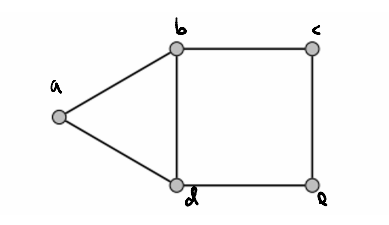
\includegraphics[width=3in]{p1.png}
            \end{center}
            \textbf{Answer}: If we label the vertices as above and let $x$ be the number of available colors, vertex $a$ has $x$ choices. Then vertex $b$ has $x-1$ choices and vertex $c$ also has $x-1$ choices. Similarly, vertex $d$ now has $x-2$ choices and so does vertex $e$. Therefore the chromatic polynomial is $p(x)=x(x-1)^2(x-2)^2$ with chromatic number $3$ (smallest number to achieve nonzero $p(x)$).
      \item [P2] Prove the following statement: For any graph $G$, the degree of its chromatic polynomial is equal to the number of vertices of $G$. (Hint: Use induction on the number of edges).\\
            \textbf{Answer}: Take a graph $G$, let $n=\abs{V}$ and $m=\abs{E}$. We will prove the statement by induction as follows:\\
            Base case: $m=1$; for the pair of connected vertices, we have $x(x-1)$ number of ways of coloring them. Each of the rest of the $n-2$ vertices can be colored $x$ ways, so the chromatic polynomial is $P(G,x)=x^{n-1}(x-1)$ which has degree $n$.\\
            Inductive step: Assume the statement holds for $m$ edges, we want to show that it will also hold for $m+1$ edges. By the Fundamental Reduction Theorem, for any pair of vertices $u,v$, and $P(G,x)=P(G-uv,x)-P(G/uv,x)$. By induction hypothesis, $P(G-uv,x)$ is a degree $n$ polynomial whereas $P(G/uv,x)$ is a degree $n-1$ polynomial. Then $P(G,x)$ has to be degree $n$.\\
            Therefore for any graph $G$, the degree of its chromatic polynomial is equal to the number of vertices of $G$ by mathematical induction.
      \item [P3] What is the chromatic number of the graph obtained from $K_n$ by removing one edge? Explain.\\
            \textbf{Answer}: $K_n$ requires a different color for each vertex, i.e. $K_n$ has a chromatic number of $n$. Then, removing one edge allows the vertices connected by the removed edge to have the same color, which means the new graph has a chromatic number of $n-1$.
\end{itemize}
\end{document}